\documentclass{article}
\usepackage{float}
\usepackage[pdftex]{graphicx}
\usepackage{listings}
\usepackage{xcolor}
\lstset{basicstyle=\ttfamily,
  showstringspaces=false,
  commentstyle=\color{red},
  keywordstyle=\color{blue}
}
\begin{document}

\author{Jon Robison}
\title{CS595 Assignment 9}
\maketitle

Q1.\\
Create a blog-term matrix. Start by grabbing 100 blogs.\\*

After writing a program to grab some given number of blogs,\\
the given generatefeedvector provided the matrix. Another program,\\
generateMatrix.py, was written to accomplish the same task, however,\\
it was noted on the slides in a sneaky location that code was provided\\
accomplishing the same thing. Much frustration at self ensued.\\
See Appendix A for program to generate bloglist, generateUrls.py\\*

Q2.\\
Create an ASCII and JPEG dendrogram that clusters (i.e., HAC)\\
the most similar blogs.\\*

The first step is always making sure this is believable to the person \\
assigning grades, and sure enough, F-Measure is beside The Living \\
Rockumentary. My grade for this assignment can go up to 11, you know.\\*

Similar blogs are grouped together, most notably, technology blogs and meta-\\
type blogs. Meta type blogs as used here are blogs about either blogging,\\
commentary (on life, ideals and culture), the meaninglessness of commentary,\\
or the meaninglessness of blogging. I found these to be most interesting, as\\
often the bloggers portray themselves as outsiders looking in to a culture\\
they appreciate, don't understand, don't connect with, are mad at, however,\\
their proximity in the dendrogram indicates they are at least similar to each\\
other. This implies there is a large subculture of people thinking they are\\
unique as an inherently positive attribute. Notable that it is (almost) the\\
majority group of this dataset, ultra large sample size that it is\\
(/hyperbole).\\*

\graphicspath{{q1/}}
\begin{figure}[H]
  \centering
  \caption{Dendrogram}
  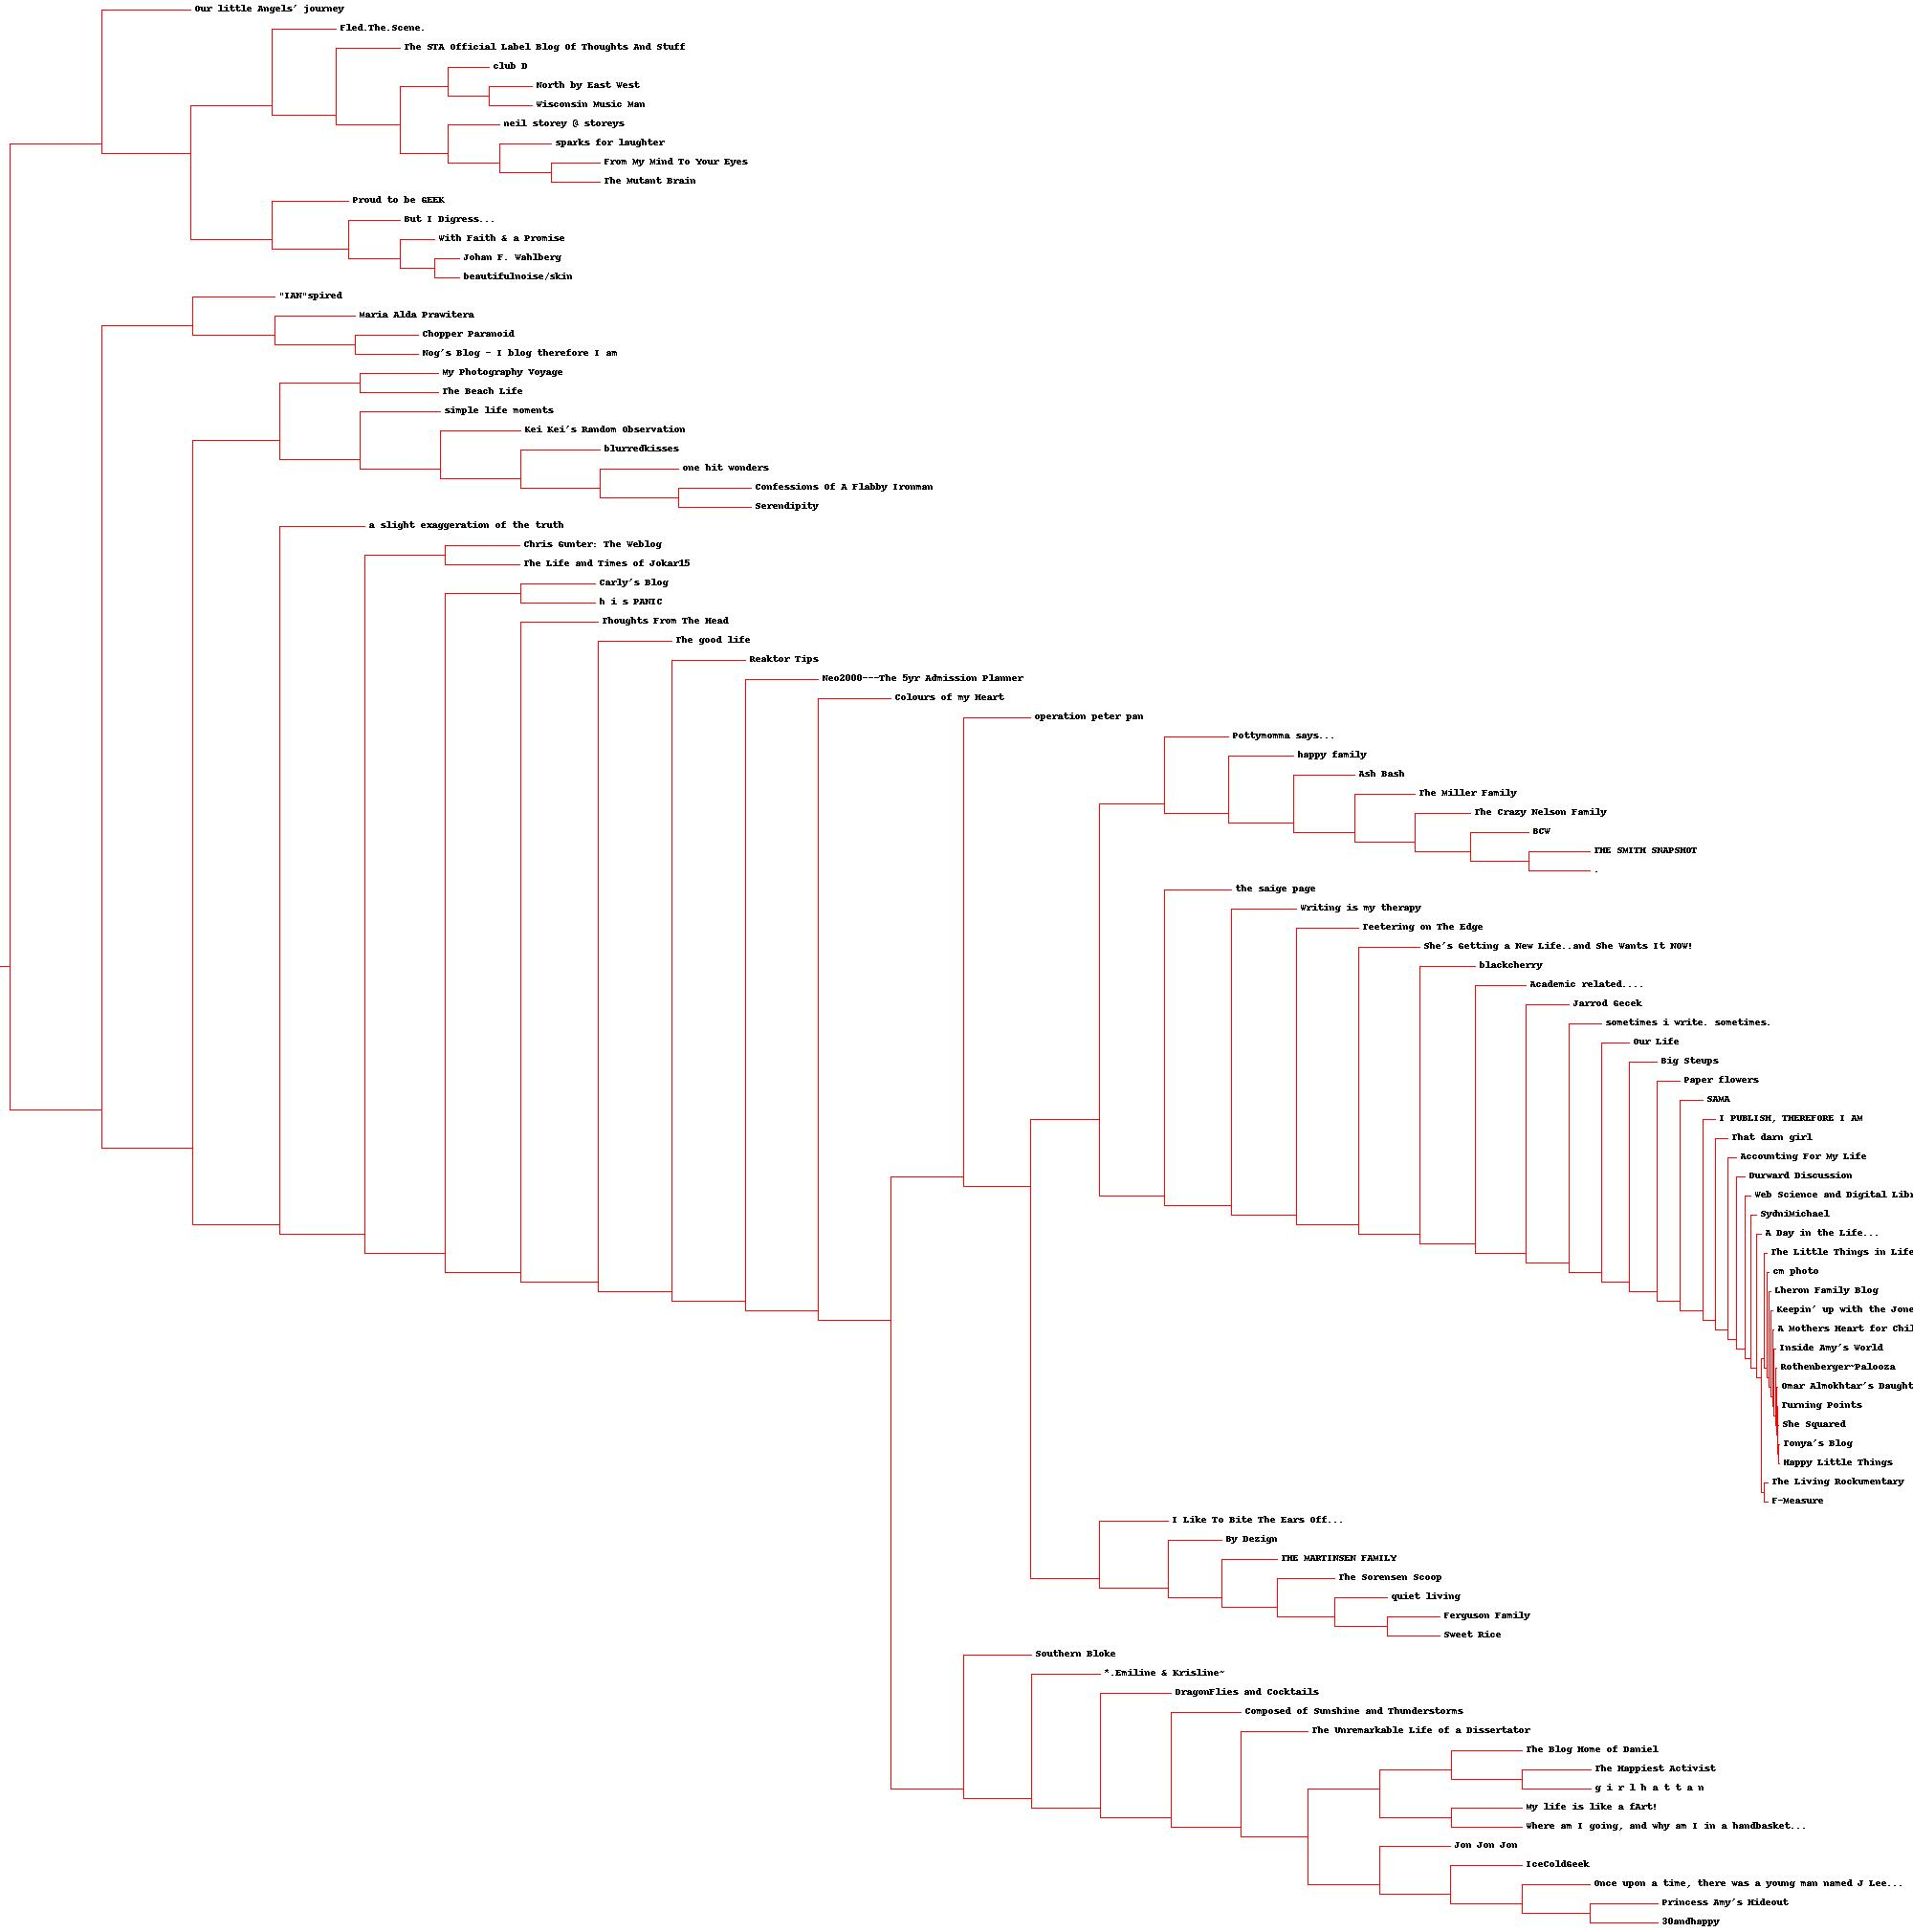
\includegraphics[scale=.2]{dendrogram.jpg}
\end{figure}
\clearpage

Q3.\\
Cluster the blogs using K-Means, using k=5,10,20. (see slide 18).\\
How many interations were required for each value of k?\\*
\begin{tabular}{c c}\\
K & Iterations\\
5 & 5\\
10 & 7\\
20 & 7\\
\end{tabular}
\\*

Q4.\\
Use MDS to create a JPEG of the blogs similar to slide 29.\\
How many iterations were required?\\*

Only one iteration before error started increasing by a factor of ten.\\
TODO This is odd and I mean to go back to see why, haven't yet.\\*

\graphicspath{{q1/}}
\begin{figure}[H]
  \centering
  \caption{Clustered Blogs}
  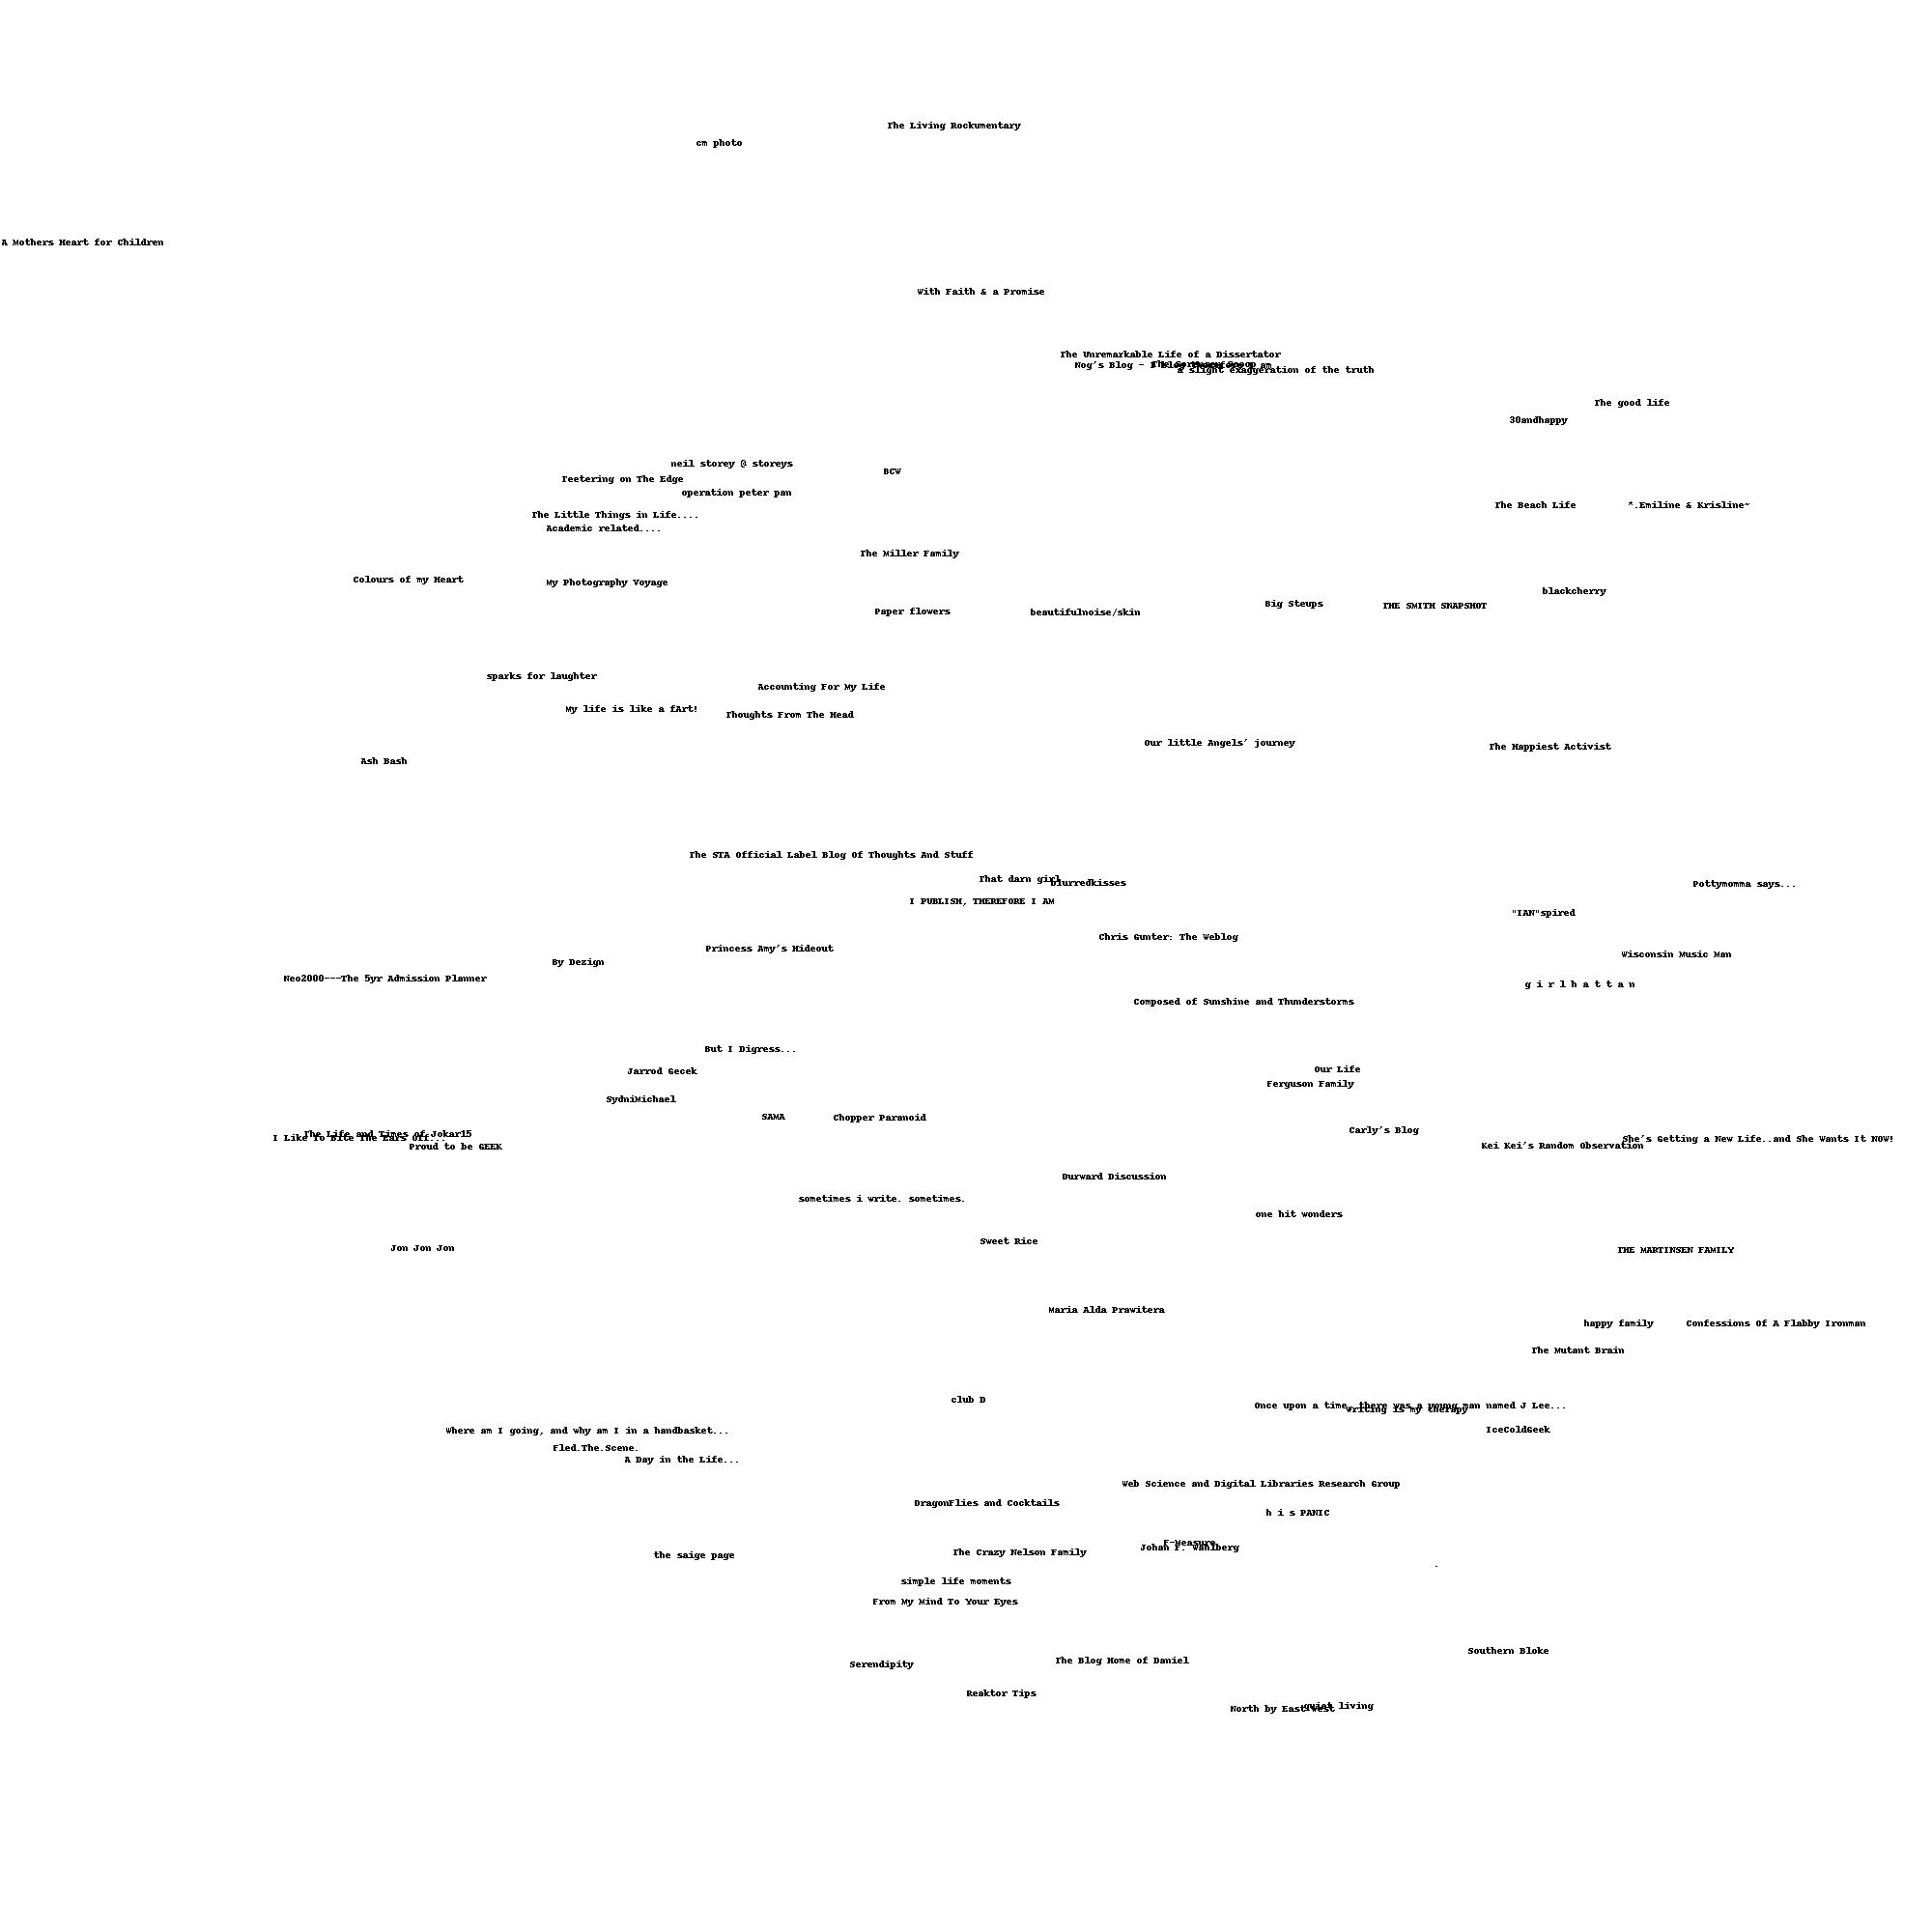
\includegraphics[scale=.2]{blogs2d.jpg}
\end{figure}
\clearpage

\appendix
\newpage
Appendix A
\lstinputlisting[language=python]{q1/generateUrls.py}
\end{document}
